
\documentclass{beamer}
\usepackage{graphicx}

\title{\texttt{thorin} and other debuggers}
\author{Ajay Tatachar}
\institute{GLUG}
\date{2021}

\begin{document}

\frame{\titlepage}

\begin{frame}
\frametitle{\texttt{thorin}?}
\begin{enumerate}
\item{A debugger for C programs}
\item{Written in Rust and C}
\item{For x86\_64 Linux and macOS}
\item{Named after this guy:}
\end{enumerate}

\begin{center}

\includegraphics[height=4cm]{thorin}\\
Figure 1.0: Thorin Oakenshield
\end{center}

\end{frame}

\begin{frame}
\frametitle{Demo!}
\end{frame}

\begin{frame}
\frametitle{\texttt{thorin}}
\begin{enumerate}
\item{Like GDB but much simpler}
\item{Reads DWARF-formatted debug info}
\end{enumerate}
\end{frame}

\begin{frame}
\frametitle{How do debuggers work?}

\begin{columns}
\begin{column}{0.48\textwidth}
Static analysis:
\begin{enumerate}
\item{DWARF debug info}
\item{Source code}
\item{Other stuff in object files}
\end{enumerate}
\end{column}
\begin{column}{0.48\textwidth}
Dynamic program interaction:
\begin{enumerate}
\item{Read the register state and memory of a running program}
\item{Inject code to set breakpoints}
\item{Step through instructions, add hooks to syscalls, etc.}
\end{enumerate}
\end{column}
\end{columns}
\end{frame}

\begin{frame}
\frametitle{DWARF}
\begin{columns}
\begin{column}{0.48\textwidth}
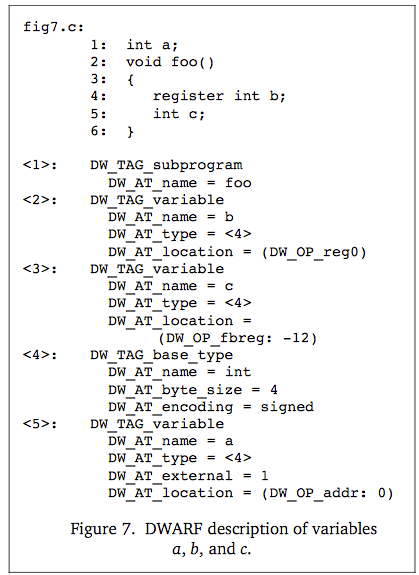
\includegraphics[height=6cm]{dwarf}
\end{column}
\begin{column}{0.48\textwidth}
\begin{enumerate}
\item{A big tree of compilation units, functions and blocks}
\item{Each ``scope'' has an associated instruction pointer range}
\item{Variable nodes are associated with scopes and encode location as absolute addresses or base-pointer offsets.}
\item{User-defined types are associated with base types or a list of members}
\end{enumerate}
\end{column}
\end{columns}
\end{frame}

\begin{frame}
\frametitle{Interacting with running programs}
Using the \texttt{ptrace} syscall:
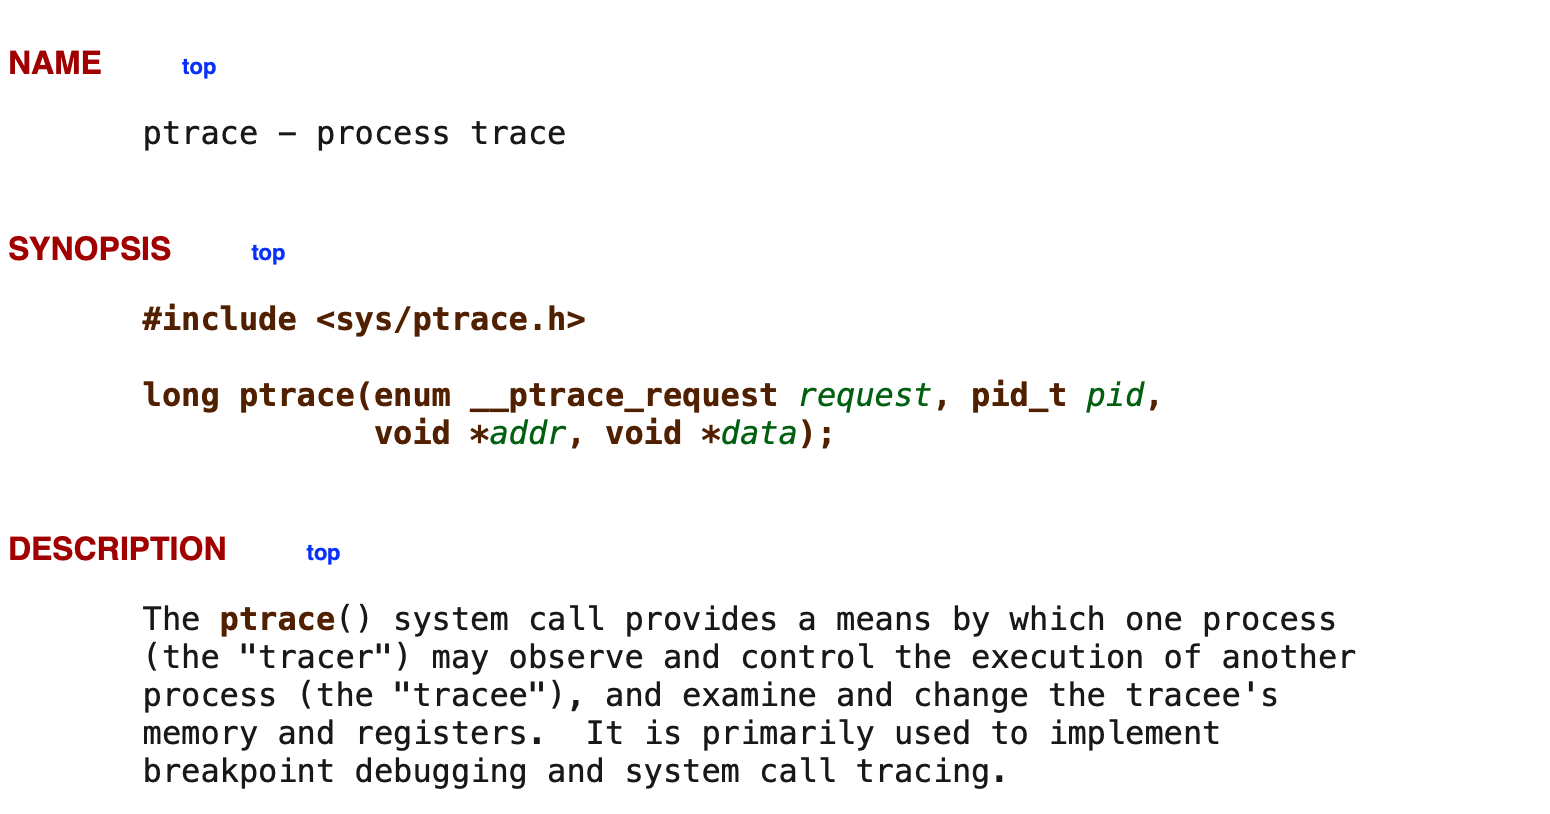
\includegraphics[height=6cm]{ptrace}
\end{frame}

\begin{frame}
\frametitle{How does thorin work?}
\begin{enumerate}
\item{Read DWARF info from object file}
\item{Construct a scope tree with IP-ranges and associated variables and types}
\item{Run the program and \texttt{ptrace} it}
\item{Wait for a segfault/abort/etc.}
\item{Figure out where we are in the scope tree and what variables we can access based on registers}
\end{enumerate}
\end{frame}

\begin{frame}
\frametitle{Misc. things}
\begin{enumerate}
\item{I had to disable ASLR when starting child processes}
\item{
Rust is difficult and not always worth it
\begin{enumerate}
\item{But pattern matching and macros are great}
\end{enumerate}
}
\item{
gdb and lldb are very powerful; this is just a small toy
\begin{enumerate}
\item{but it was a great learning experience in systems programming}
\end{enumerate}
}
\end{enumerate}
\end{frame}

\end{document}